%% LyX 2.2.3 created this file.  For more info, see http://www.lyx.org/.
%% Do not edit unless you really know what you are doing.
\documentclass[12pt,english]{article}
\usepackage[osf]{mathpazo}
\renewcommand{\sfdefault}{lmss}
\renewcommand{\ttdefault}{lmtt}
\usepackage[T1]{fontenc}
\usepackage[latin9]{inputenc}
\usepackage[paperwidth=30cm,paperheight=35cm]{geometry}
\geometry{verbose,tmargin=2cm,bmargin=2cm}
\setlength{\parindent}{0bp}
\usepackage{amsmath}
\usepackage{amssymb}

\makeatletter
%%%%%%%%%%%%%%%%%%%%%%%%%%%%%% User specified LaTeX commands.
\usepackage{tikz}
\usetikzlibrary{matrix,arrows,decorations.pathmorphing}
\usetikzlibrary{shapes.geometric}
\usepackage{tikz-cd}
\usepackage{amsthm}
\usepackage{xparse,etoolbox}

\theoremstyle{plain}
\newtheorem{theorem}{Theorem}[section]
\newtheorem{lemma}[theorem]{Lemma}
\newtheorem{prop}{Proposition}[section]
\newtheorem*{cor}{Corollary}
\theoremstyle{definition}
\newtheorem{defn}{Definition}[section]
\newtheorem{ex}{Exercise} 
\newtheorem{example}{Example}[section]
\theoremstyle{remark}
\newtheorem*{rem}{Remark}
\newtheorem*{note}{Note}
\newtheorem{case}{Case}
\usepackage{graphicx}
\usepackage{amssymb}
\usepackage{tikz-cd}
\usetikzlibrary{calc,arrows,decorations.pathreplacing}
\tikzset{mydot/.style={circle,fill,inner sep=1.5pt},
commutative diagrams/.cd,
  arrow style=tikz,
  diagrams={>=latex},
}

\usepackage{babel}
\usepackage{hyperref}
\hypersetup{
    colorlinks,
    citecolor=blue,
    filecolor=blue,
    linkcolor=blue,
    urlcolor=blue
}
\usepackage{pgfplots}
\usetikzlibrary{decorations.markings}
\pgfplotsset{compat=1.9}


\newcommand{\blocktheorem}[1]{%
  \csletcs{old#1}{#1}% Store \begin
  \csletcs{endold#1}{end#1}% Store \end
  \RenewDocumentEnvironment{#1}{o}
    {\par\addvspace{1.5ex}
     \noindent\begin{minipage}{\textwidth}
     \IfNoValueTF{##1}
       {\csuse{old#1}}
       {\csuse{old#1}[##1]}}
    {\csuse{endold#1}
     \end{minipage}
     \par\addvspace{1.5ex}}
}

\raggedbottom

\blocktheorem{theorem}% Make theo into a block
\blocktheorem{defn}% Make defi into a block
\blocktheorem{lemma}% Make lem into a block
\blocktheorem{rem}% Make rem into a block
\blocktheorem{cor}% Make col into a block
\blocktheorem{prop}% Make prop into a block


\usepackage[bottom]{footmisc}

\makeatother

\usepackage{babel}
\begin{document}

\title{Calculating $H(S_{I})$ when $I$ is a Monomial Ideal}

\maketitle
\begin{lemma}\label{lemmadim0monomialideal} Suppose $I$ is a monomial
ideal and let $\mathcal{M}=\{m_{1},\dots,m_{r}\}$ be the unique minimal
basis of $I$. For each $\lambda=1,\dots,n$, let $k_{\lambda}$ be
a nonnegative even integer such that $x_{\lambda}^{k_{\lambda}}$
does not divide any monomial in $\mathcal{M}$. Then 
\[
H(S_{I})\cong H(S_{I+\langle x_{1}^{k_{1}},\dots,x_{n}^{k_{n}}\rangle}).
\]

\end{lemma}

\begin{proof} We prove by induction on $\lambda=1,\dots,n$. The
base case $\lambda=1$ will follow if $H(S_{I:x_{1}^{k_{1}}})\cong0$,
since 
\[
H(S_{I})\cong H(S_{I:x_{1}^{k_{1}}})\oplus H(S_{\langle I,x_{1}^{k_{1}}\rangle}).
\]
by Theorem~(\ref{theoremdecomposition}). Since $x_{1}^{k_{1}}$ does
not divide any monomial in $\mathcal{M}$, a basis for $I:x_{1}^{k_{1}}$
is given by $\mathcal{M}'=\{m_{1}',\dots,m_{r}'\}$, where if $m_{\mu}=x_{1}^{\alpha_{\mu1}}x_{2}^{\alpha_{\mu2}}\cdots x_{n}^{\alpha_{\mu n}}$,
then $m_{\mu}'=x_{2}^{\alpha_{\mu2}}\cdots x_{n}^{\alpha_{\mu n}}$
for all $\mu=1,\dots,r$. In particular, if $f\in S_{I:x_{1}^{k_{1}}}$
represents a cycle in $H(S_{I:x_{1}^{k_{1}}})$, then $x_{1}f\in S_{I:x_{1}^{k_{1}}}$
represents a boundary of $f$ in $H(S_{I:x_{1}^{k_{1}}})$. Thus $H(S_{I:x_{1}^{k_{1}}})=0$,
and our claim is proved. 

~~~For the induction step, assume that 
\[
H(S_{I})\cong H(S_{\langle I,x_{1}^{k_{1}},\dots,x_{\lambda}^{k_{\lambda}}\rangle})
\]
for some $1\leq\lambda<n$. By the same argument as in the base case
(with $\langle I,x_{1}^{k_{1}},\dots,x_{\lambda}^{k_{\lambda}}\rangle$
replaced with $I$), we have $H(S_{\langle I,x_{1}^{k_{1}},\dots,x_{\lambda}^{k_{\lambda}}\rangle:x_{\lambda+1}^{k_{\lambda+1}}}\cong0.$
Thus
\begin{align*}
H(S_{I}) & \cong H(S_{\langle I,x_{1}^{k_{1}},\dots,x_{\lambda}^{k_{\lambda}}\rangle})\\
 & \cong H(S_{\langle I,x_{1}^{k_{1}},\dots,x_{\lambda}^{k_{\lambda}}\rangle:x_{\lambda+1}^{k_{\lambda+1}}})\oplus H(S_{\langle I,x_{1}^{k_{1}},\dots,x_{\lambda}^{k_{\lambda}},x_{\lambda+1}^{k_{\lambda+1}}\rangle})\\
 & \cong H(S_{\langle I,x_{1}^{k_{1}},\dots,x_{\lambda}^{k_{\lambda}},x_{\lambda+1}^{k_{\lambda+1}}\rangle})
\end{align*}

\end{proof}

\begin{example}\label{example} Consider $S=K[x,y]$ and $I=\langle x^{3},x^{2}y\rangle$.
Setting $J=I+\langle x^{4},y^{2}\rangle$, Proposition~(\ref{propdim0monomialideal})
tells us that $H(S_{I})\cong H(S_{J})$. There is a nice topological
picture associated with $S_{J}$. 

\begin{center}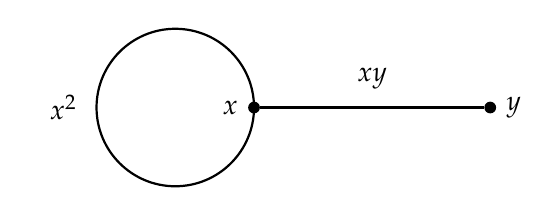
\begin{tikzpicture}

\draw[thick] (0,0) circle (1cm);

\node[circle, fill=black, inner sep=1.5pt, label=left:$x$] (x) at (1,0) {};

\node[circle, fill=black, inner sep=1.5pt, label=right:$y$] (y) at (4,0) {};

\node[circle, inner sep=1.5pt, label=below:$xy$] (z) at (2.5,0.7) {};

\node[circle, inner sep=1.5pt, label=right:$x^2 $] (w) at (-1.8,0) {};

\draw[thick] (x) -- (y); 



\end{tikzpicture}\end{center} 

\end{example}

\subsection{Delta Complex}

We now want to generalize the Stanley-Reisner construction. Suppose
$I$ is a monomial ideal. We denote by $\Delta_{I}$ to be the $\Delta$-set
which consists of sets of the form 
\[
S_{k}:=\{\text{monomials of degree }k\text{ which are not in }I\}=(S_{I})_{k}
\]
for all $k\geq0$, and which consists of face maps $\sigma_{i}:S_{k}\to S_{k-1}$,
given by deleting the $i$th term of a monomial. We recover the differential
$d_{k}$ from the formula
\[
d_{k}:=\sum_{i=1}^{k}\sigma_{i}
\]

\begin{example}\label{example} (Delta Complex of Torus) Consider
$S=K[x,y]$ and $I=\langle x^{2},y^{2}\rangle$. \end{example}
\end{document}
